\chapter{Introduction}

Here we introduce and familiarise with the basic definitions and notations about Cellular Automata, a tool dating back to the late 1940s, when Stanislaw Ulam and John von Neumann defined it as a model for natural and biological processes.

\section{Cellular Automaton}
\label{ca}

A cellular automaton (abbrev. CA) is a discrete dynamical system consisting of cells that change their states simultaneously according a local update rule. This update process is repeated at discrete time steps.
Cellular automata are\cite{canotes}

\begin{itemize}
	\item discrete in space and time,
	\item homogeneous in space and time,
	\item local in their interactions.
\end{itemize}


\paragraph{Basics}

Let:

\begin{itemize}

	\item $\mathds{Z}^{d}$ be a $d$-dimensional cellular space, with $d \in \mathds{N}^{+}$. Elements of this set are called \textit{cells}.

	\item $S$ be a finite state set. Elements of this set are called \textit{states}.

	\item $c$ be a \textit{configuration} of a d-dimensional CA with a state set S, defined as the following function:

	$$c: \mathds{Z}^d \rightarrow S$$
	that assigns a state to each cell.

	\item $c(\vec{n })$ the state of a cell $\vec{n} \in \mathds{Z}^d$

\end{itemize}

Most frequently we consider one and two-dimensional spaces, in which cases the cells from a line are indexed by $\mathds{Z}$ (line) or by $\mathds{Z}^2$ (grid).

Denoting the set of functions from set A from B with $B^A$ we can write that the set of all configurations is $S^{\mathds{Z}^d}$.

A d-dimensional neighborhood vector of size m is a tuple

$$N = N = (\vec{n}_1,\vec{n}_2,...,\vec{n}_m) $$

where each $\vec{n}_i \in \mathds{Z}^d$ and $\vec{n}_i \neq \vec{n}_j$ for all $i \neq j$.

The \textit{local update rule} of a CA with state set S and size m neighborhood is a fuction

$$ f: S^m \rightarrow S$$

specifying the new state of the cell based on the old states of its neighborhood.

As we mentioned, all cells use the same rule, and this rule is applied simultaneously. Global configuration $c$ becomes $c'$ where for all $\vec{n} \in \mathds{Z}^n$:

$$c'(\vec{n}) = f[c(\vec{n}, \vec{n}_1),c(\vec{n}, \vec{n}_2), ... , c(\vec{n}, \vec{n}_m)]$$

$c \mapsto c' $ is our \textit{global transition function} $G: S^{\mathds{Z}^d} \longrightarrow S^{\mathds{Z}^d}$. Typically, G is iterated to produce a time evolution of the system.

$$ c \mapsto G(c) \mapsto G^2(c) \mapsto G^2(c) \mapsto..$$

\paragraph{Formal definition}

A CA is a 4-tuple $A=(d, S,N,f)$ where

\begin{itemize}
	\item d is the dimension,
	\item S is the finite state set,
	\item N is the neighborhood vector,
	\item f is the local update rule.

\end{itemize}

\subsection{Neighborhoods}
Regarding the two-dimensional CAs, there are two fundamental types of neighbourhoods that are mainly considered:
\begin{itemize}
	\item von Neumann neighbourhood, that consists of the central cell, whose condition is to be updated, and the four cells located to the north, south, east and west of the central cell
	\item Moore neighbourhood, that consists of the same cells with the von Neumann neighbourhood together with the four other adjacent cells of the central cell (the north-west, north-east, south-east and south-west cells)
\end{itemize}


\begin{figure*}
  \centering
  \subfigure[Caption A]{%
    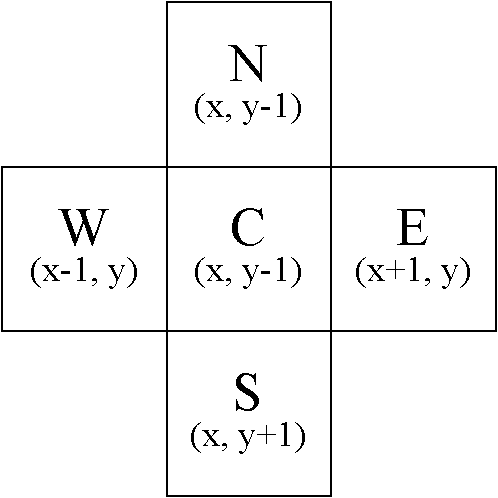
\includegraphics[width=0.23\textwidth]{vn_n}%
    \label{fig:a}%
    jjj
    }\hspace{1cm}%or more
    \subfigure[Caption B]{%
    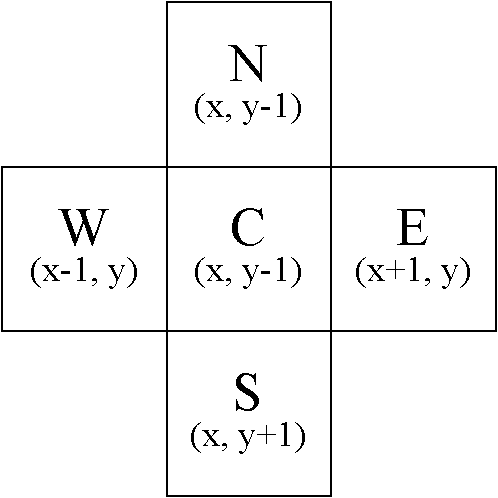
\includegraphics[width=0.228\textwidth]{vn_n}%
    \label{fig:b}%
    
  }%  
  \caption{Figure Caption}
  \label{fig:ab}
\end{figure*}


\subsection{Examples}

\par
The most known CA in the scientific literature is \textit{Game of Life}, devised by the John Horton Conway in 1970 with the intention of producing a simple model of von Neumann's idea of the machine capable of reproducing itself and simulate a Turing machine. 
\par
In the universe of \textit{Game of Life} each cell is in one of two possible states, alive or dead (or populated and unpopulated, respectively). Every cell interacts with its eight neighbours, which are the cells that are horizontally, vertically, or diagonally adjacent. At each step in time, the following transitions occur:
\begin{itemize}
	\item Any live cell with fewer than two live neighbours dies, as if by underpopulation
	\item Any live cell with two or three live neighbours lives on to the next generation
	\item Any live cell with more than three live neighbours dies, as if by overpopulation
	\item Any dead cell with exactly three live neighbours becomes a live cell, as if by reproduction
\end{itemize}
\par
The initial pattern constitutes the seed of the system. The first generation is created by applying the above rules simultaneously to every cell in the seed; births and deaths occur simultaneously, and the discrete moment at which this happens is sometimes called a tick. Each generation is a pure function of the preceding one. The rules continue to be applied repeatedly to create further generations. 

\section{Physarum}

Physarum polycephalum \cite{sun2017physarum}, \cite{mayne2016biology} is a species of order Physarales, subclass Myxogas-tromycetidae, class Myxomecetes, division Myxostelida, commonly known as a true slime mould, that inhabits shady, cool and moist areas. 
\par
Physarum thrives in favorable environmental conditions, particularly when the right combinations of humidity, temperature and nutrient presence are found. If the conditions are not adequate for development, Physarum behaves like a single-celled organism that does not demonstrate organizational skills. In appropriate conditions, it joins together to create particularly efficient filamentary nets in physical distribution.
\paragraph{Life cycle}
It is common to refer to the Physarum by the name of its vegetative (resting) life cycle phase, the plasmodium. The Physarum plasmodium is a single yellow cytoplasmic mass that can range in size from a few mm$^2$ to over half a m$^2$. The organism will typically be composed of a network of protoplasmic veins that can contain more than 100,000 nuclei.
\par
It is during this stage that the organism searches for food. Multiple sources state that the plasmodium is both predatory and saprophytic: its natural foodstuffs include fungal spores, bacteria, smaller amoebae and decaying matter, the latter of which may be digested extracellularly through the secretion of enzymes.
\par
If environmental conditions cause the plasmodium to desiccate during feeding or migration, Physarum will have another life cycle phase called the sclerotium. The sclerotium is basically highly resistant desiccated tissue that serves as a dormant stage, protecting Physarum for long periods of time. The organism will assume it if environmental conditions become too
unfavourable. Once favorable conditions resume, a sclerotium can be revert back to a viable plasmodium that reappears to continue its quest for food.
\par
As the food supply runs out, the plasmodium stops feeding and begins its reproductive phase. Stalks of sporangia form from the plasmodium. It is within these structures that meiosis occurs and spores are formed. Sporangia are usually formed in the open spaces so that the spores they release will be spread by wind currents.
\par
Spores can remain dormant for years if needed. However, when environmental conditions are favorable for growth, the spores germinate and release either flagellated or amoeboid swarm cells (motile stage). The swarm cells then fuse together to form a new plasmodium. 

